% !TeX encoding = UTF-8
% !TeX spellcheck = es_ES
% !TeX root = ComponentCatalog.tex
%!TEX root=ComponentCatalog.tex

\subsection{Conectores Jack}
% !TeX encoding = UTF-8
% !TeX spellcheck = es_ES
% !TeX root = ../ComponentCatalog.tex
%!TEX root=../ComponentCatalog.tex

%DC Jack 2 mm plastico Amazon
\begin{table}[H]
    \centering
    \renewcommand\theadfont{\bfseries}
    \setlength{\tabcolsep}{10pt}
    \renewcommand{\arraystretch}{1.5}

    \begin{tabular}{|c|c|c|c|c|}
        \beginConnectorTable{DC Jack 2mm}
        \multirow{4}{*}{\makecell{Macho \\ Plug}}
    
        \connectordata{
            \begin{scope}
                \clip (-1.3,-0.75) rectangle  +(2.6,1.5);
                \node[inner sep=0pt] at (-1.8,-0.8)
                    {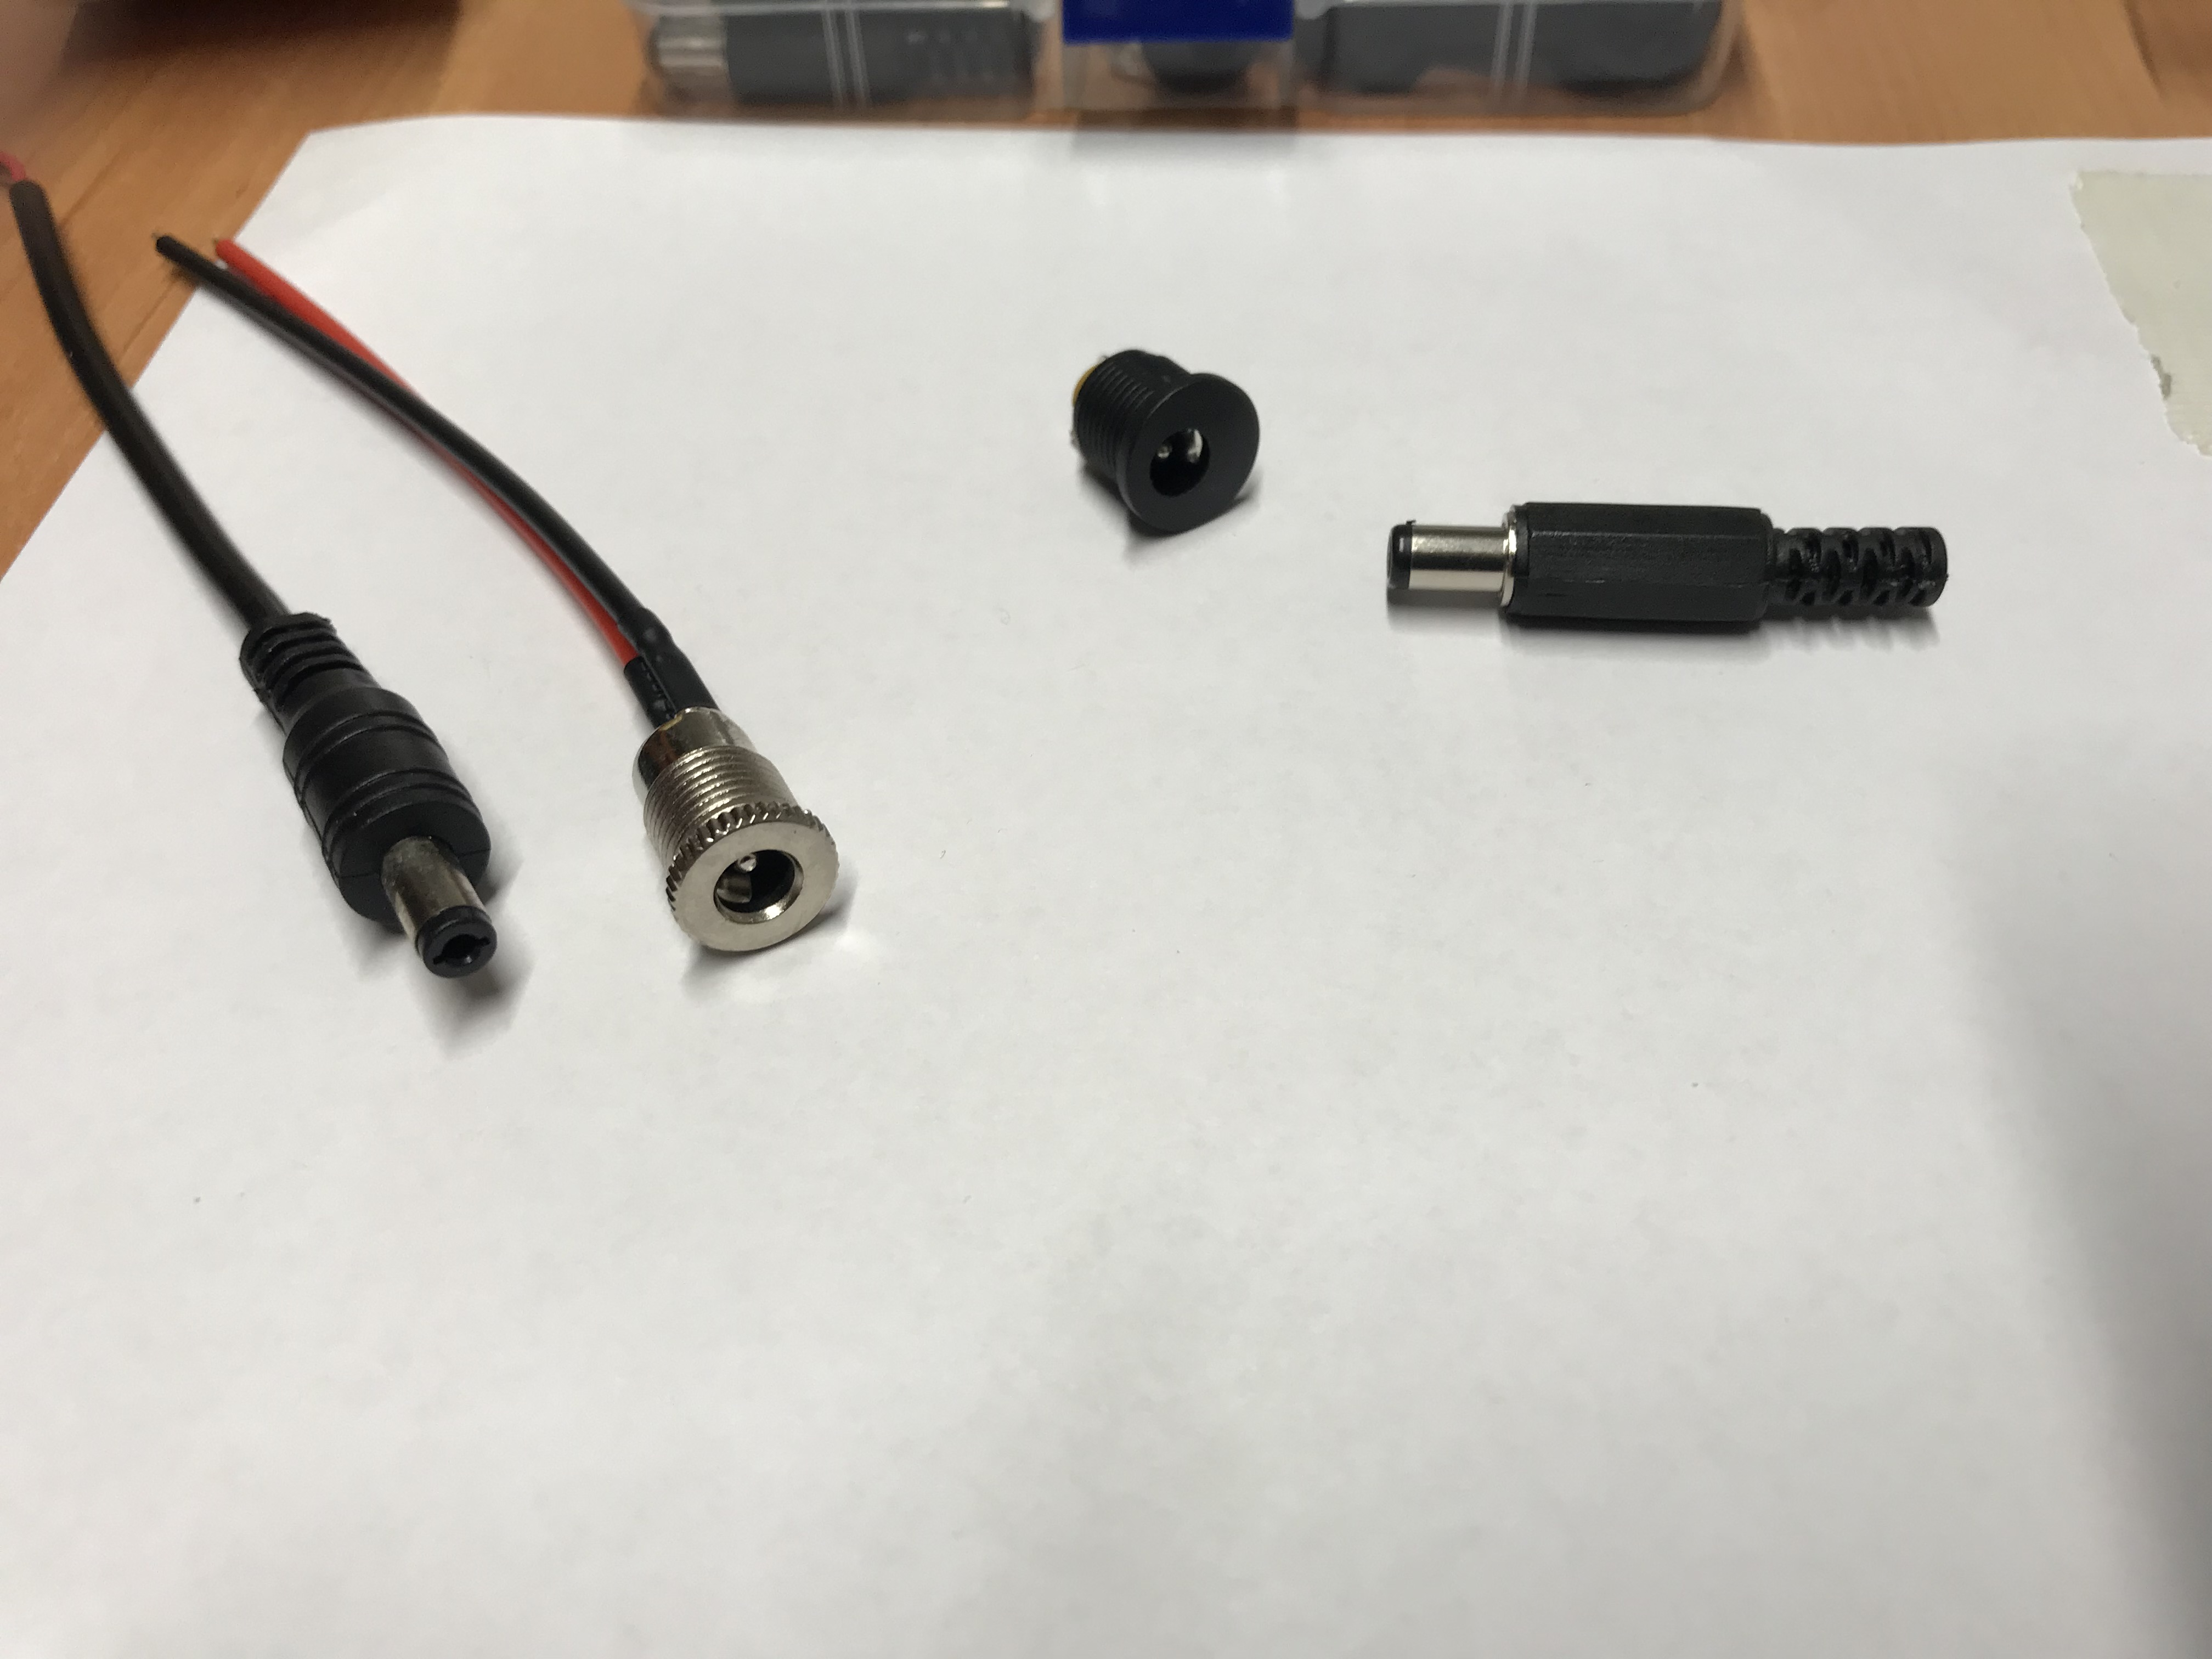
\includegraphics[scale=.05]{pictures/dcJack.jpg}};
            \end{scope}
        }{
            \draw (0,0) rectangle (3,1.5) ;
        }{Amazon}{Sin Id} {24V} {3A}
        \connectorinfo{Codigo}{ KLDX-PA-0202-A}{\tabitem \textbf{Fabricante}: Kycon}
        \cline{1 - 2}
        \multirow{4}{*}{\makecell{Hembra \\ Socket}}
        \connectordata{
            \begin{scope}
                \clip (-1,-0.75) rectangle  +(2,1.5);
                \node[inner sep=0pt] at (-0.2,-1.7)
                    {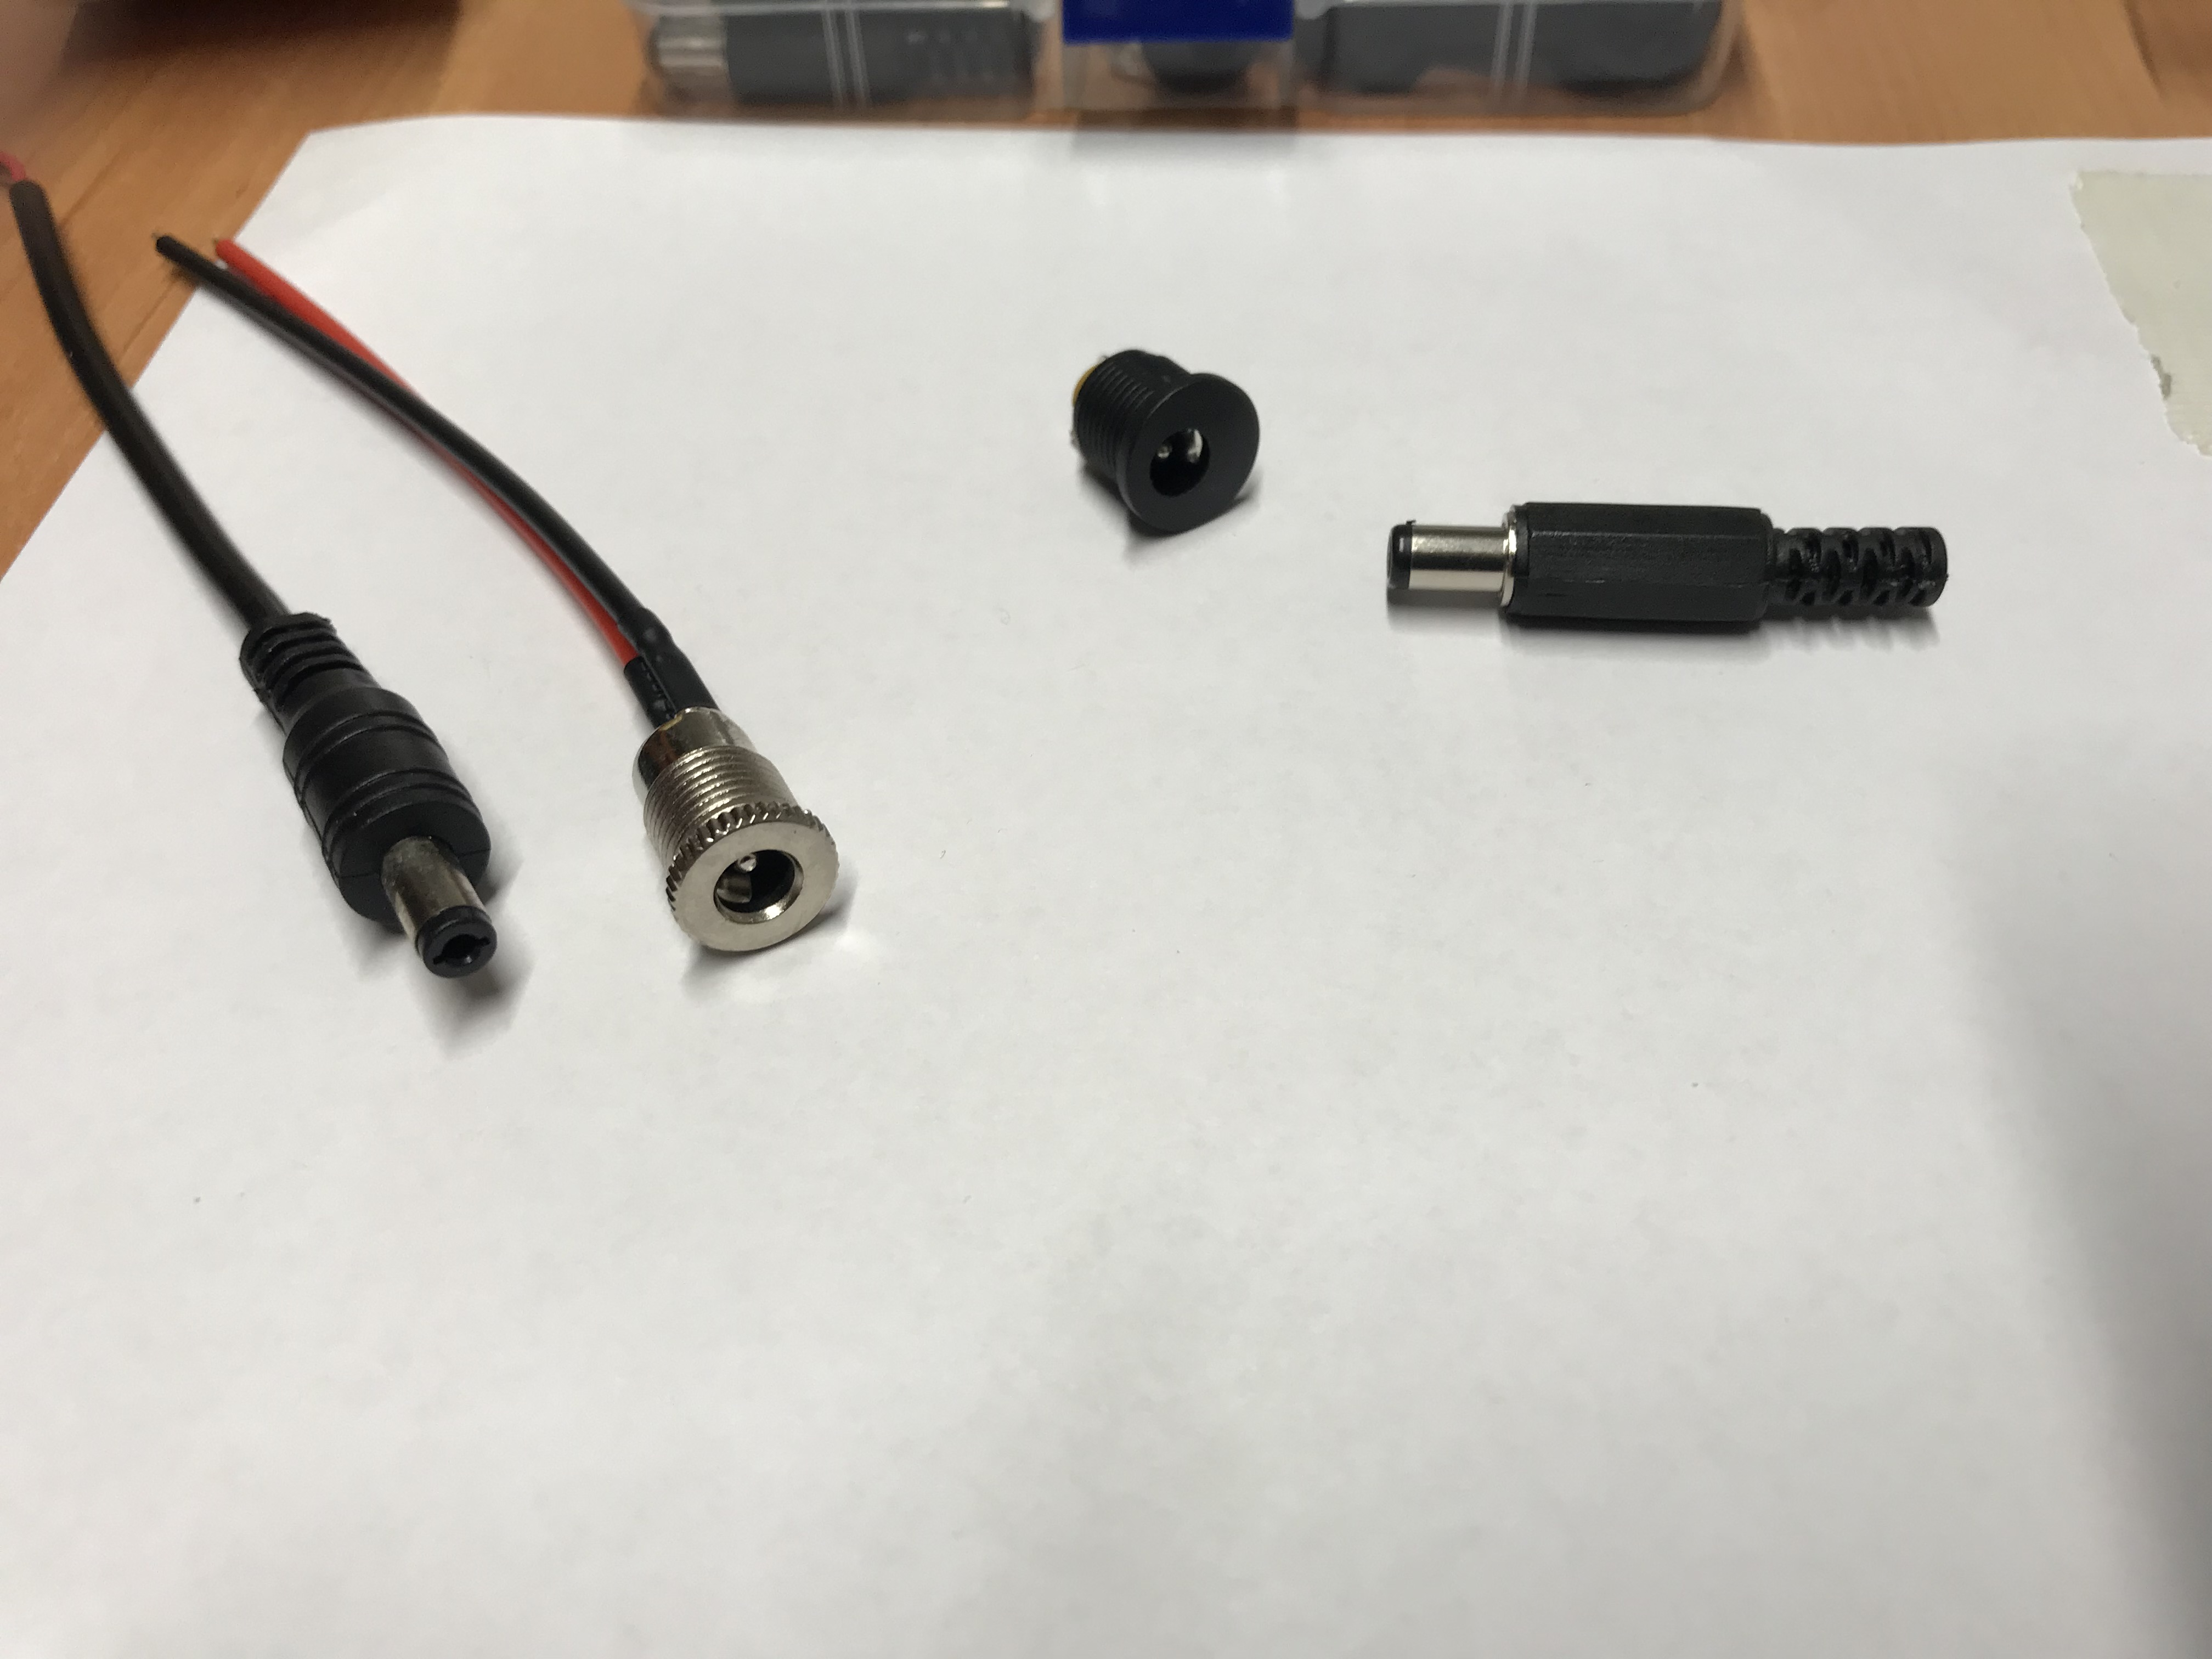
\includegraphics[scale=.07]{pictures/dcJack.jpg}};
            \end{scope}
        }{
            \draw (0,0) rectangle (3,1.5) ;
        }{Amazon}{Sin Id} {12V} {0.5A}
        \connectorinfo{Codigo}{	NEB/J 21 C}{ \tabitem \textbf{Fabricante}: LUMBERG  \\}
        \cline{1 - 2}
        
        \multicolumn{5}{|l|}{\makecell[l]{
            \tabitem Incluye tuerca para sujetar a panel \\
            \tabitem Incluye protector de goma
        }} \\
        \hline
        
        \multirow{4}{*}{\makecell{Macho \\ Plug}}
        \connectordata{
            \begin{scope}
                \clip (-1,-0.65) rectangle  +(2,1.3);
                \node[inner sep=0pt, rotate=60] at (1.3,2)
                    {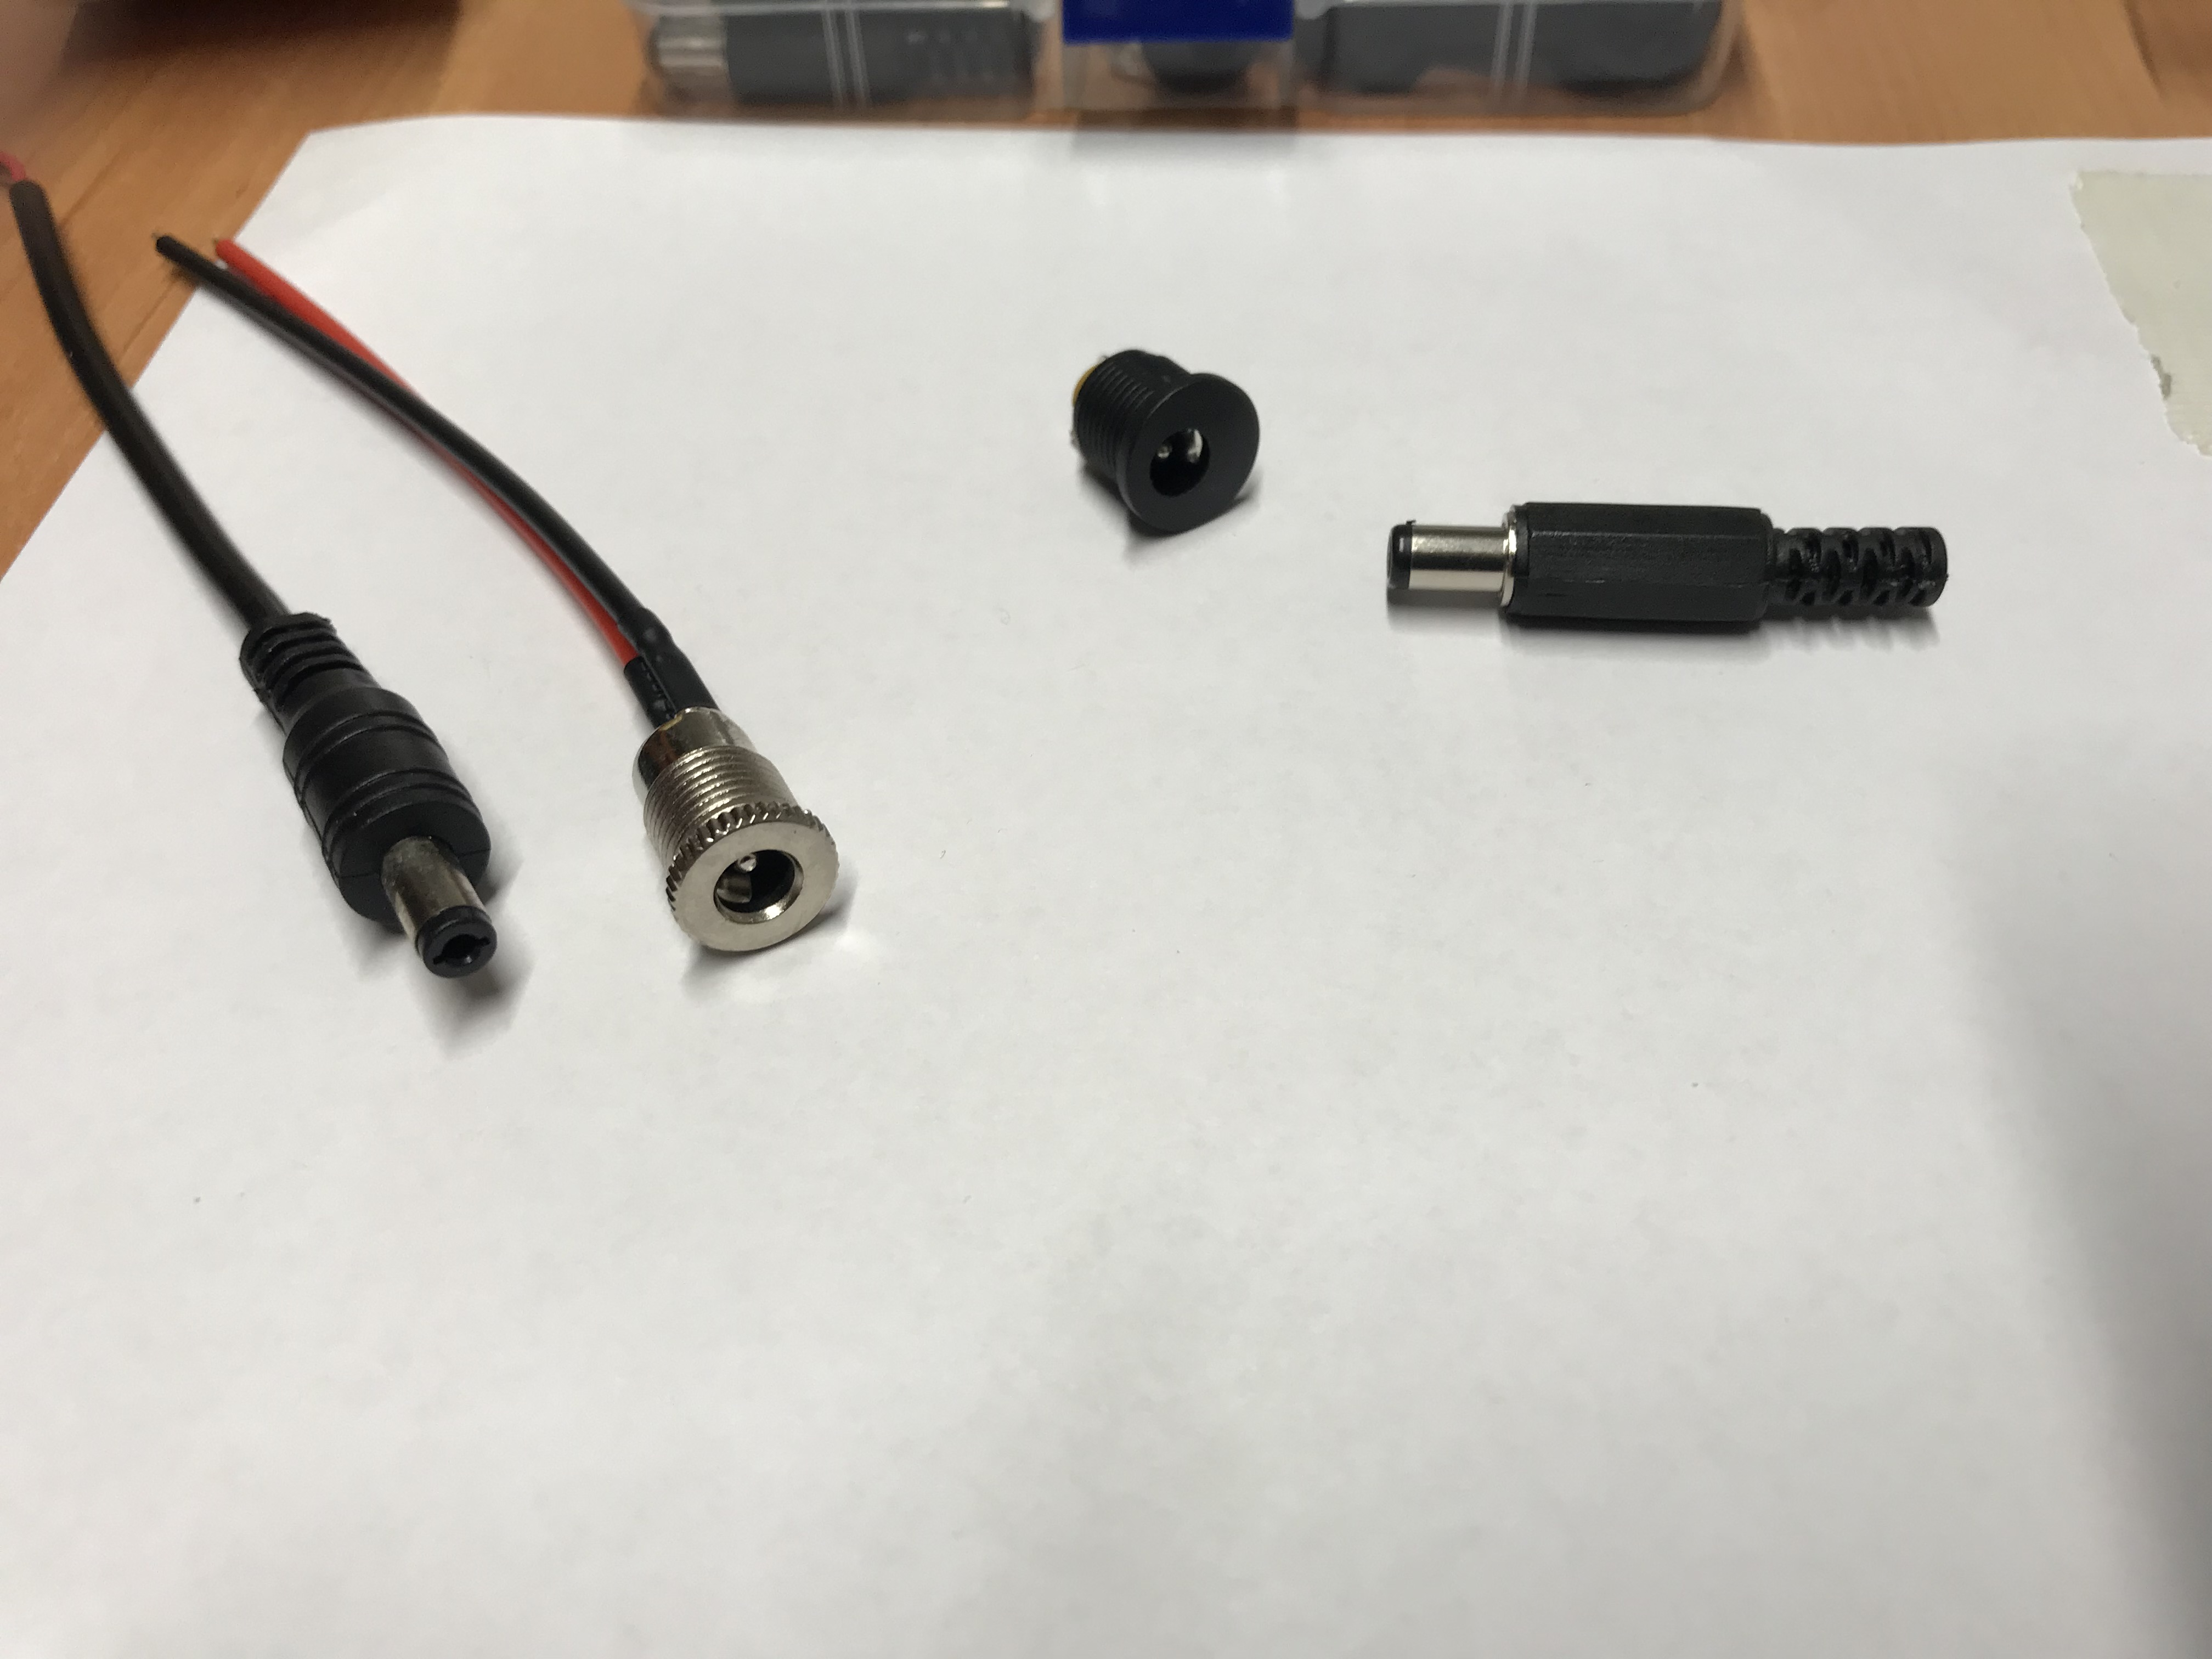
\includegraphics[scale=.05]{pictures/dcJack.jpg}};
            \end{scope}
           
        }{
            \draw (0,0) rectangle (3,1.5) ;
        }{Amazon}{Sin Id} {24V} {3A}
        %\cline{1 - 2}
        & \multicolumn{4}{|l|}{
            \tabitem Cables sobre molde
        }
        \\ \hline

        \multirow{3}{*}{\makecell{Hembra \\ Socket}}
        \connectordata{
            \begin{scope}
                \clip (-1,-0.65) rectangle  +(2,1.3);
                \node[inner sep=0pt, rotate=60] at (0.9,1)
                    {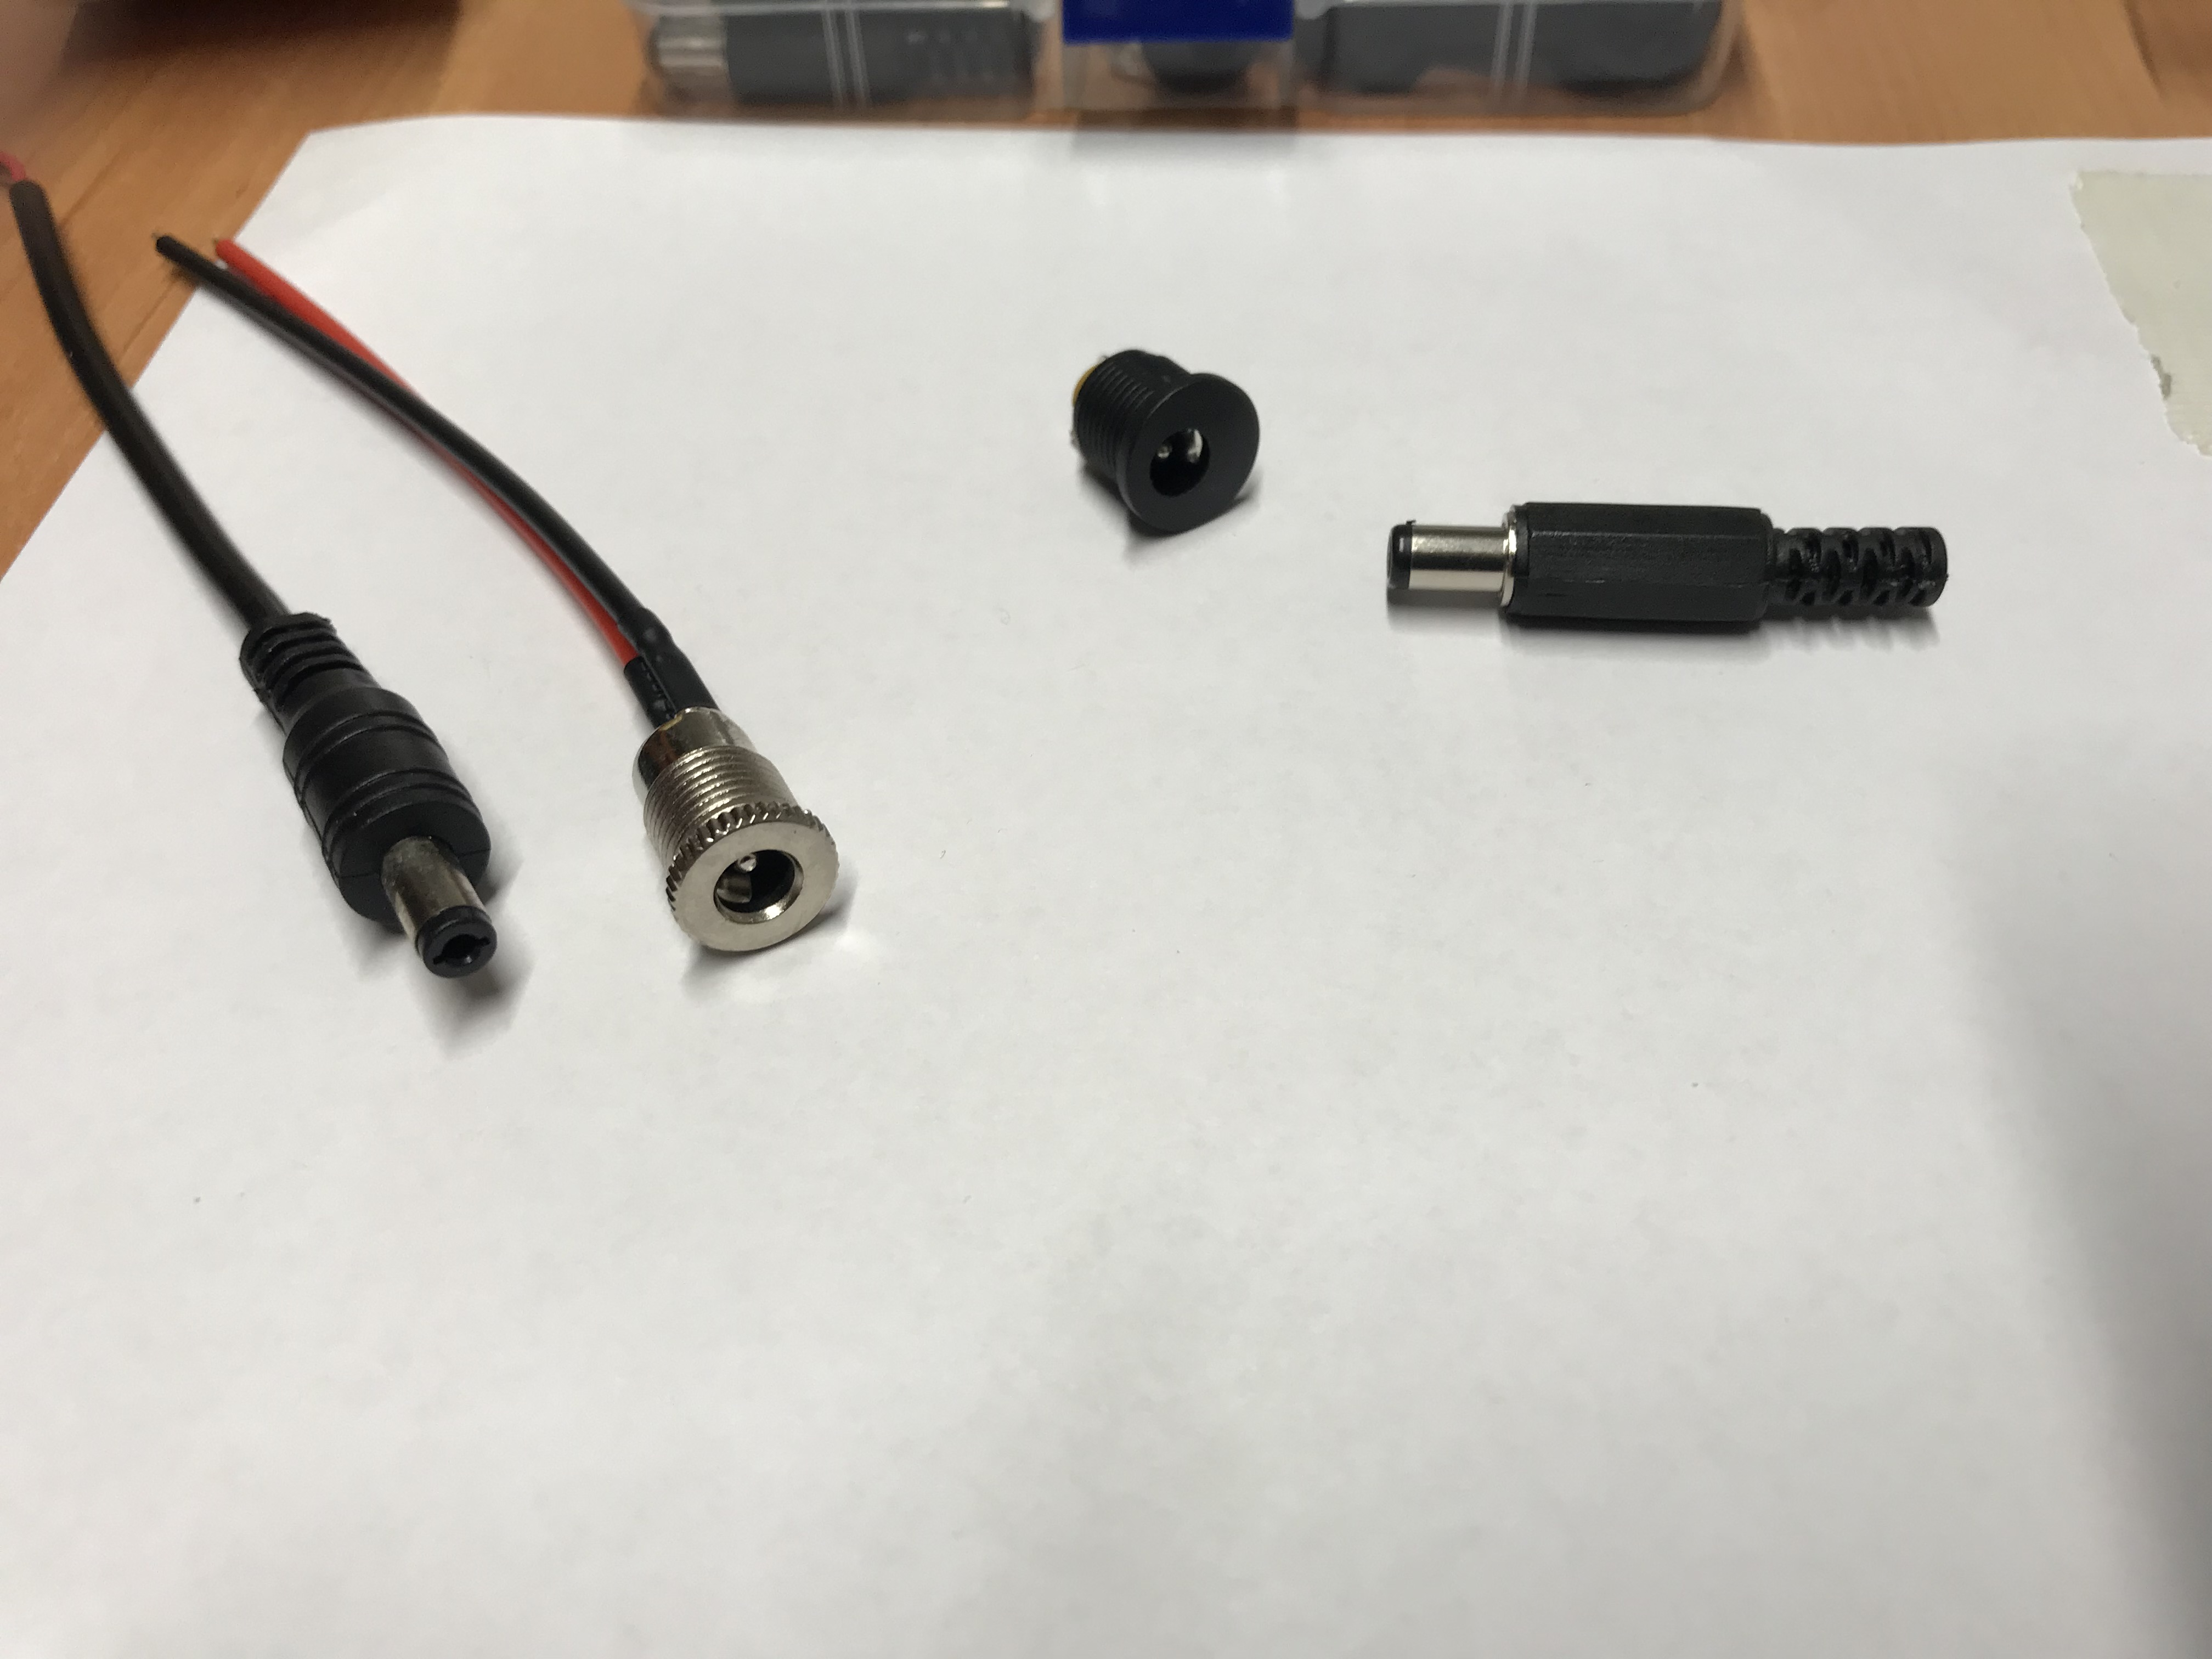
\includegraphics[scale=.05]{pictures/dcJack.jpg}};
            \end{scope}
        }{
            \draw (0,0) rectangle (3,1.5) ;
        }{Amazon}{Sin Id} {12V} {0.5A}
        \connectorinfo{Codigo}{1614 16}{ \tabitem \textbf{Fabricante}: LUMBERG  \\}
        \cline{1 - 2}
        \multicolumn{5}{|l|}{\makecell[l]{
            \tabitem Incluye tuerca para sujetar a panel \\
            \tabitem Es de metal conectado a (-) \\
            \tabitem Cables pre-soldados
        }} \\
        \hline
        \connectorblockinfo{Uso}{Paso de corriente a cajas}
        \connectorblockinfo{Ubicacion}{TR}


        \noalign{\vskip 2mm}    
        \beginConnectorTable{KLDX-0202-A Jack Para PCB}
        \multirow{4}{*}{\makecell{Hembra \\ Socket}}
        \connectordata{
            \begin{scope}
                \clip (-1,-0.75) rectangle  +(2,1.5);
                \node[inner sep=0pt] at (0,0)
                    {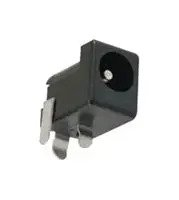
\includegraphics[scale=.35]{pictures/connectors/KLDX-0202-A.jpg}};
            \end{scope}
        }{
            \draw (0,0) rectangle (3,1.5) ;
        }{Mouser}{KLDX-0202} {24V} {3.5A}
        
        \connectorinfo{Codigo}{KLDX-0202-A}{
            \tabitem \textbf{Fabricante}: Kycon
        }
        \cline{1 - 2}
        %\hline
        \connectorblockinfo{Uso}{Paso de corriente a PCB}
        \connectorblockinfo{Ubicacion}{CJ}
    \end{tabular}
    \caption{Jack 2mm}
    \label{tab:DcJackPcb2mm}
\end{table}


\subsection{Conectores JST}
% !TeX encoding = UTF-8
% !TeX spellcheck = es_ES
% !TeX root = ../ComponentCatalog.tex
%!TEX root=../ComponentCatalog.tex

%RCY
\begin{table}[H]
    \centering
    \renewcommand\theadfont{\bfseries}
    \setlength{\tabcolsep}{10pt}
    \renewcommand{\arraystretch}{1.5}

    \begin{tabular}{|c|c|c|c|c|}
        \beginConnectorTable{JST RCY 2 Vias}
        \multirow{5}{*}{\makecell{Macho \\ Plug }}

        \connectordata{
            \begin{scope}
                \clip (0,0) rectangle  +(3,1.5);
                \node[inner sep=0pt] at (-1.9,1.7)
                    {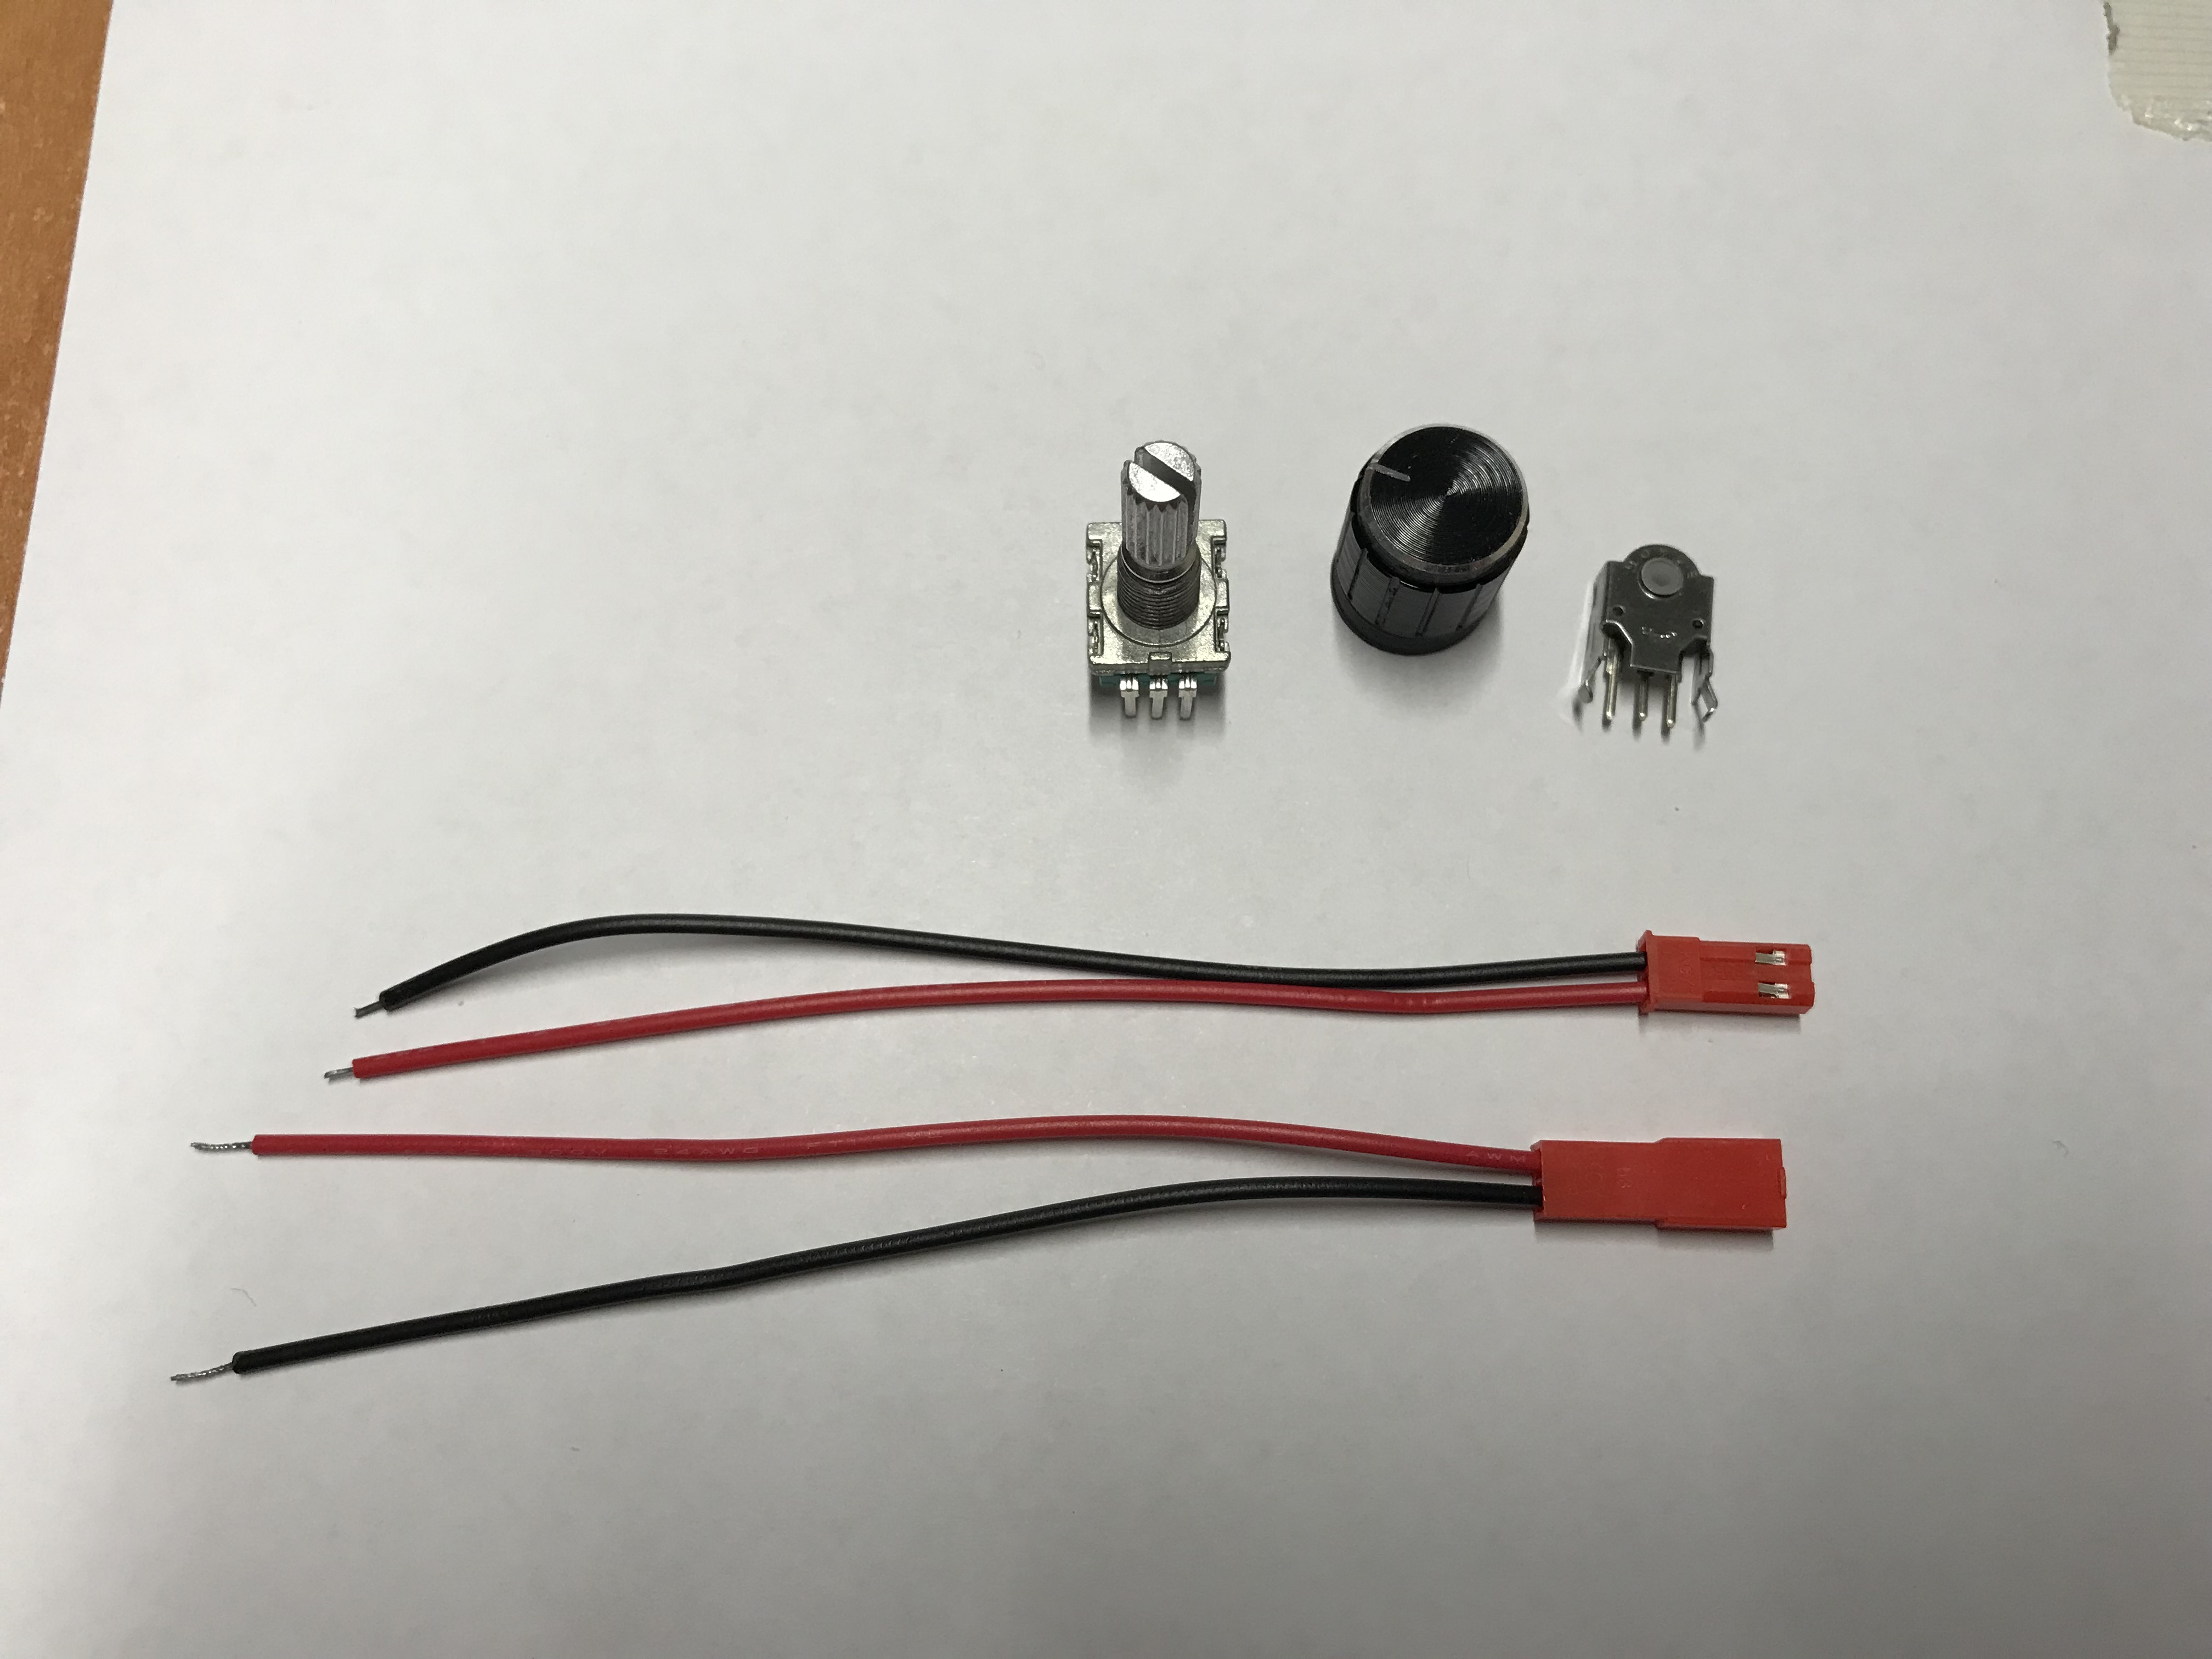
\includegraphics[scale=.1]{pictures/JST.jpg}};
            \end{scope}
        }{
            \draw (0,0) rectangle (3,1.5) ;
        }{Aliexpress}{JST RCY} {250V} {3A} 
        
        \connectorinfo{Housing}{SYP-02T-1}{
            \tabitem \textbf{Tipo}: Plug  \\
             \tabitem \textbf{Color}: Rojo
        }
        \connectorinfo{Contact}{SYF-001T-P0.6}{
            \tabitem \textbf{Tipo}: Socket  \\
            \tabitem \textbf{AWG}: 22-28 \\
            \tabitem \textit{Alternativa}:	BYF-001T-P0.6
        } 
        \cline{1 - 2}

        \multirow{3}{*}{\makecell{Hembra \\ Socket}}
        \connectordata{
            \begin{scope}
                \clip (0,0) rectangle  +(3,1.5);
                \node[inner sep=0pt] at (-1.8,3)
                    {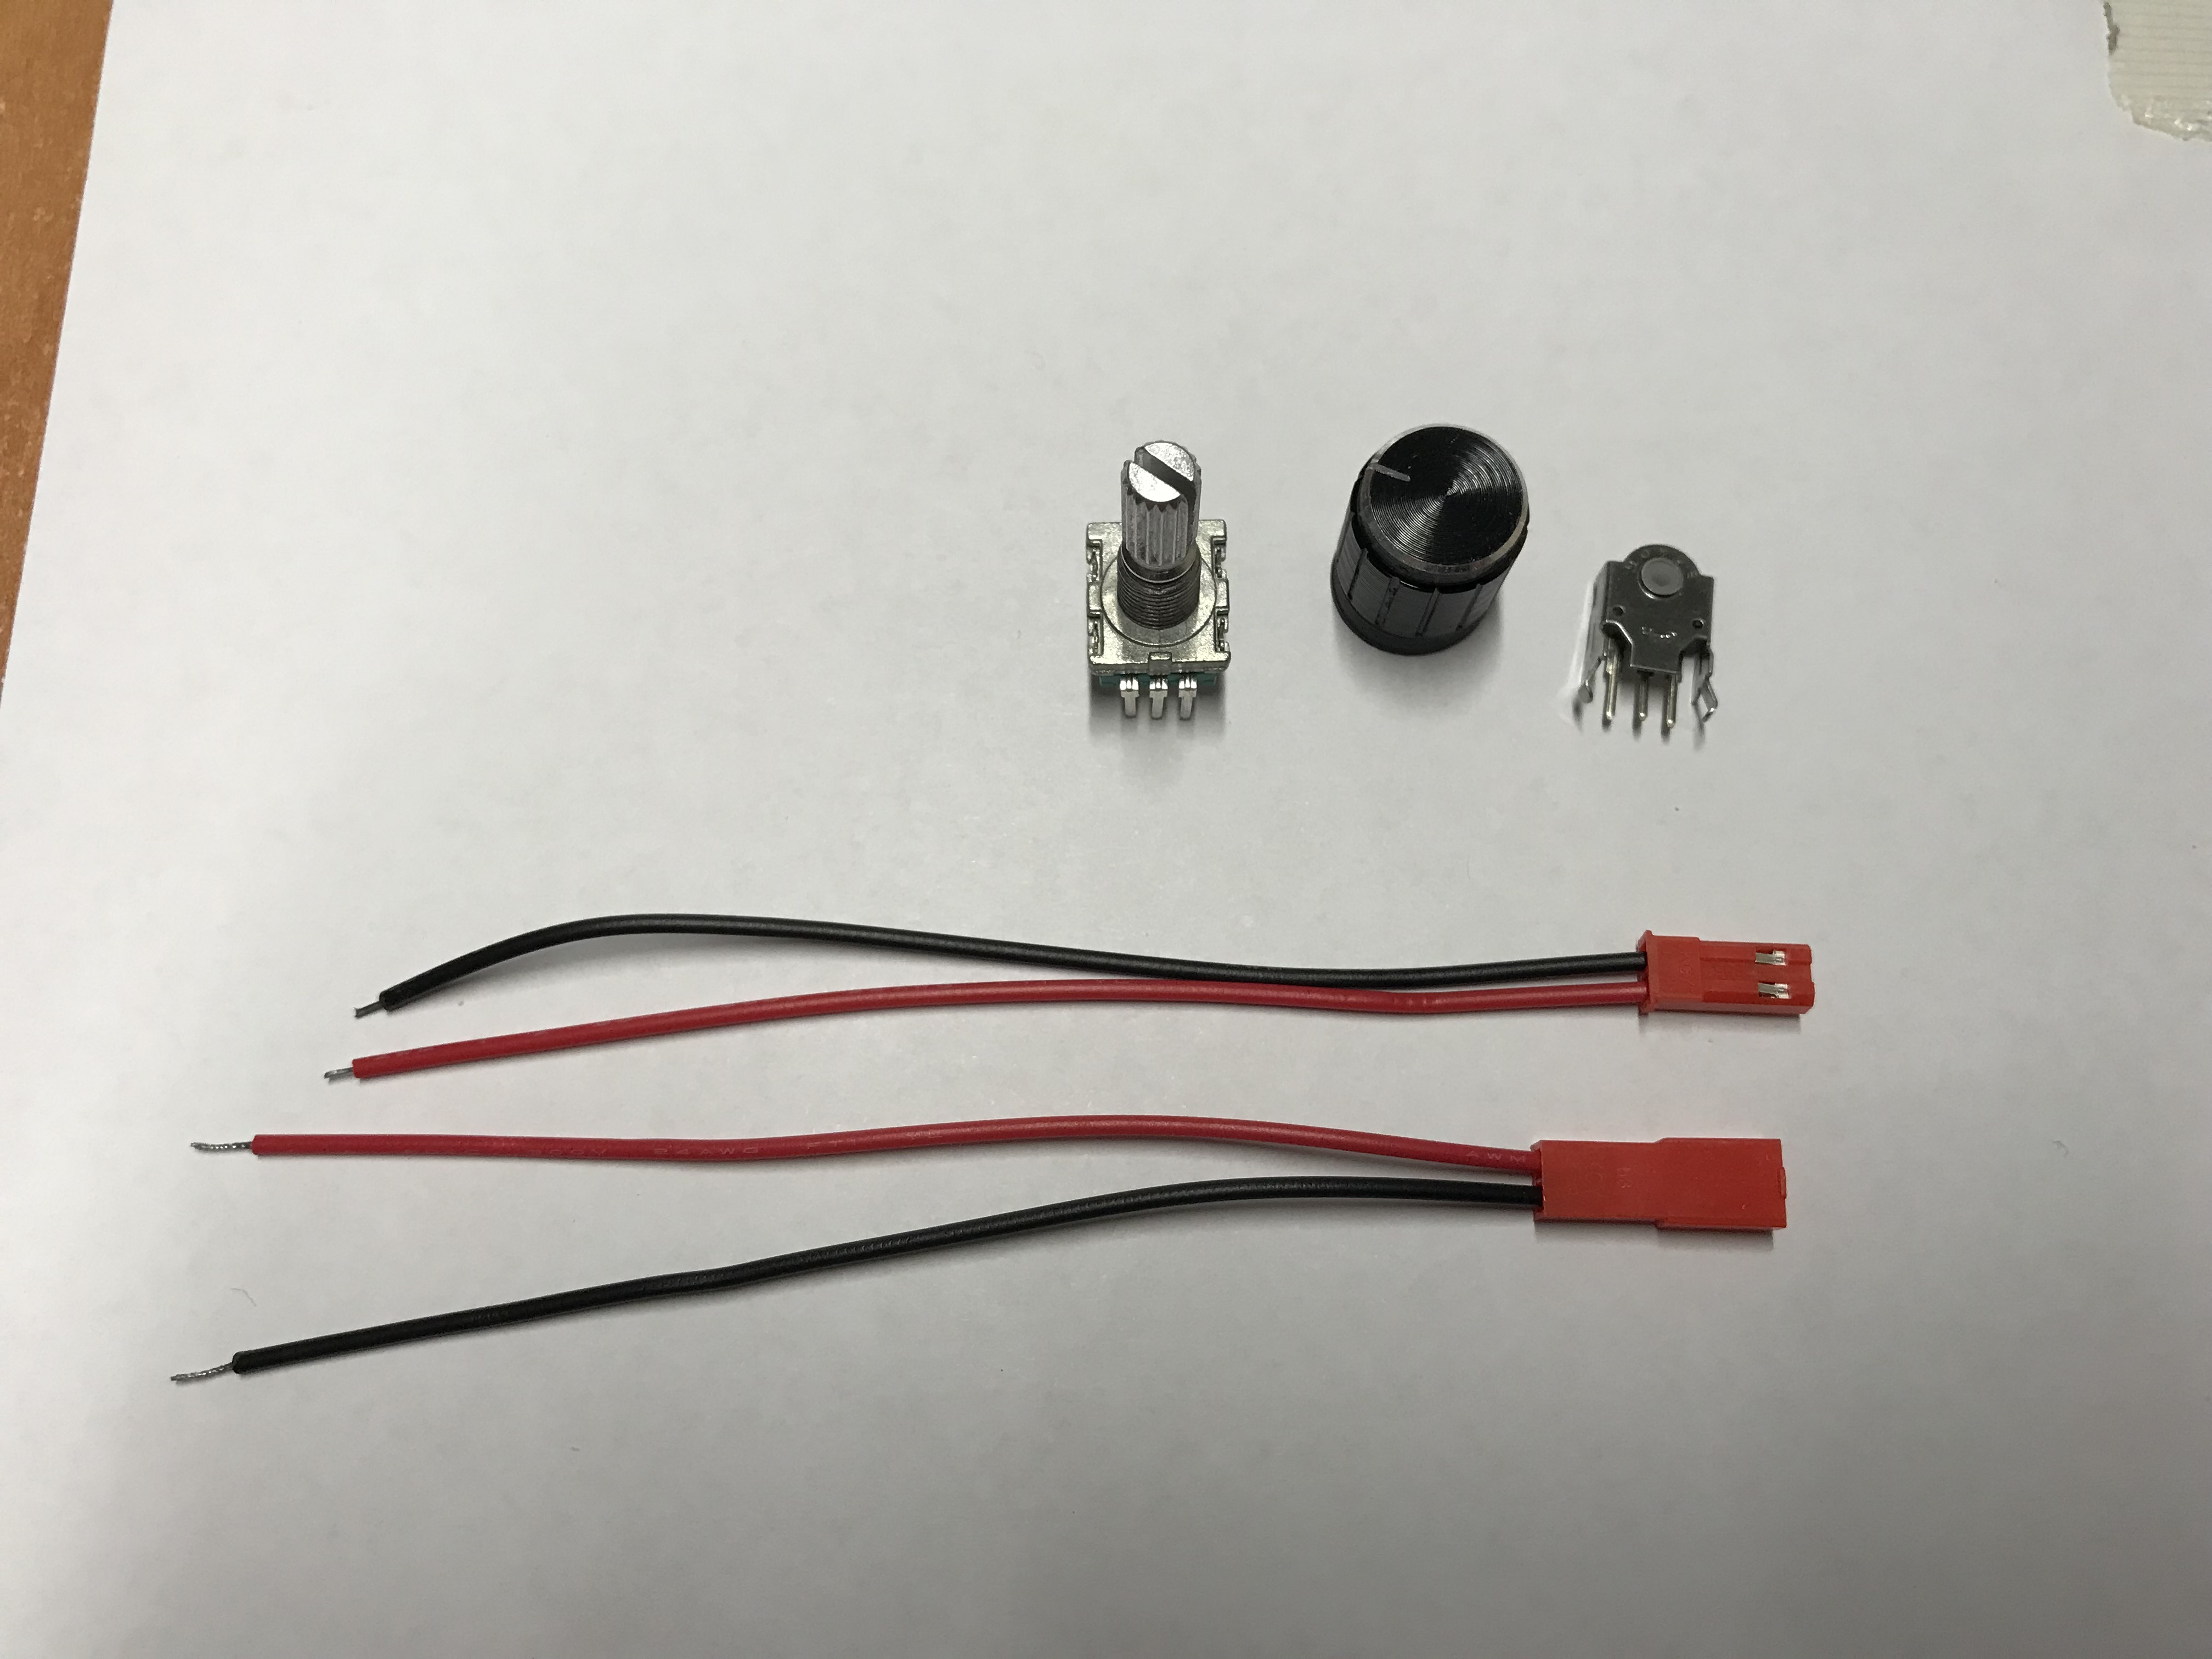
\includegraphics[scale=.1]{pictures/JST.jpg}};
            \end{scope}
        }{
            \draw (0,0) rectangle (3,1.5) ;
        }{Aliexpress}{JST RCY} {250V} {3A}
        \connectorinfo{Housing}{SYR-02T}{
            \tabitem \textbf{Tipo}: Receptacle  \\
             \tabitem \textbf{Color}: Rojo
        }
        \connectorinfo{Contact}{SYM-001T-P0.6}{
            \tabitem \textbf{Tipo}: Pin  \\
            \tabitem \textbf{AWG}: 22-28 \\
            \tabitem \textit{Alternativa}: BYM-001T-P0.6
        }
        \cline{1 - 2}
        \multicolumn{5}{|l|}{\makecell[l]{
            \tabitem Incluyen cables presoldados
        }} \\
        \hline
        \connectorblockinfo{Uso}{Paso de corriente entre modulos}
        \connectorblockinfo{Ubicacion}{TT-Tren}
    \end{tabular}
    \caption{JST RCY}
    \label{tab:DcJstRcy}
\end{table}

\begin{table}[H]
    \centering
    \renewcommand\theadfont{\bfseries}
    \setlength{\tabcolsep}{10pt}
    \renewcommand{\arraystretch}{1.5}

    \begin{tabular}{|c|c|c|c|c|}
        \beginConnectorTable{JST SM 3 Vias}
        \multirow{5}{*}{\makecell{Macho \\ Plug }}

        \connectordata{     
            \begin{scope}
                \clip (0,0) rectangle  +(2,1.5);
                \node[inner sep=0pt] at (-1.2,1.2)
                    {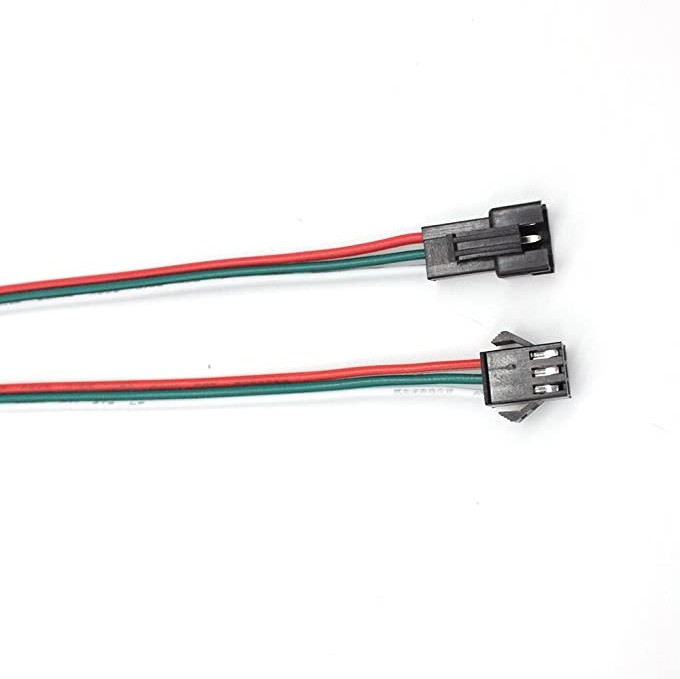
\includegraphics[scale=0.5]{pictures/connectors/jst-sm.jpg}};
            \end{scope}
        }{
            \draw (0,0) rectangle (3,1.5) ;
        }{Amazon}{JST SM} {250V} {3A} 
        
        \connectorinfo{Housing}{SMP-03V-BC}{
            \tabitem \textbf{Tipo}: Plug  \\
             \tabitem \textbf{Color}: Negro
        }
        \connectorinfo{Contact}{SHF-001T-0.8BS}{
            \tabitem \textbf{Tipo}: Socket  \\
            \tabitem \textbf{AWG}: 22-28 \\
            \tabitem \textit{Alternativa}: BHF-001T-0.8BS
        } 
        \cline{1 - 2}

        \multirow{3}{*}{\makecell{Hembra \\ Socket}}
        \connectordata{
            \begin{scope}
                \clip (0,0) rectangle  +(2.2,1.5);
                \node[inner sep=0pt] at (-0.8,-0.55)
                    {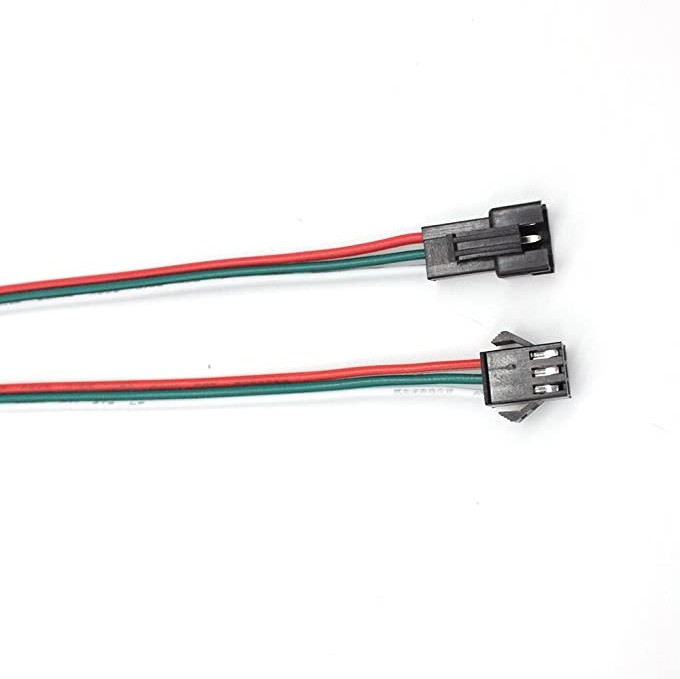
\includegraphics[scale=0.5]{pictures/connectors/jst-sm.jpg}};
            \end{scope}
        }{
            \draw (0,0) rectangle (3,1.5) ;
        }{Amazon}{JST SM} {250V} {3A}
        \connectorinfo{Housing}{SMR-03V-B}{
            \tabitem \textbf{Tipo}: Receptacle  \\
             \tabitem \textbf{Color}: Rojo
        }
        \connectorinfo{Contact}{SYM-001T-P0.6}{
            \tabitem \textbf{Tipo}: Pin  \\
            \tabitem \textbf{AWG}: 22-28 \\
            \tabitem \textit{Alternativa}: BYM-001T-P0.6
        }
        \cline{1 - 2}
        \multicolumn{5}{|l|}{\makecell[l]{
            \tabitem Incluyen cables presoldados
        }} \\
        \hline
        \connectorblockinfo{Uso}{Conexion NeoPixel}
        \connectorblockinfo{Ubicacion}{TT-Tren}
    \end{tabular}
    \caption{JST RCY}
    \label{tab:DcJstSM}
\end{table}

{
    \renewcommand{\arraystretch}{1.5}
    \renewcommand\theadfont{\bfseries}
    \setlength{\tabcolsep}{10pt}
    \begin{longtable}[H]{|c|c|c|c|c|}
    %\centering


        \beginConnectorTable{JST XH}
        \multirow{10}{*}{\makecell{Macho \\ Plug }}
        \connectorinfo{Contact}{SXH-001T-P0.6}{
            \tabitem \textbf{Tipo}: Socket  \\
            \tabitem \textbf{AWG}: 22-28 \\
            \tabitem \textit{Alternativa}: BXH-001T-P0.6
        } 

        \connectordata{     
            \begin{scope}
                \clip (0,0) rectangle  +(3,1.5);
                \node[inner sep=0pt] at (1.5,0.75)
                    {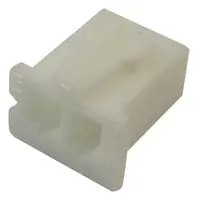
\includegraphics[scale=0.4]{pictures/connectors/XH/XHP-2.jpg}};
            \end{scope}
        }{
            \draw (0,0) rectangle (3,1.5) ;
        }{Farnell}{JST XH} {250V} {3A} 
        
        \connectorinfo{Housing}{XHP-2}{
            \tabitem \textbf{Tipo}: Plug  \\
             \tabitem \textbf{Color}: Blanco
        }

        \connectordata{     
            \begin{scope}
                \clip (0,0) rectangle  +(3,1.5);
                \node[inner sep=0pt] at (1.5,0.75)
                    {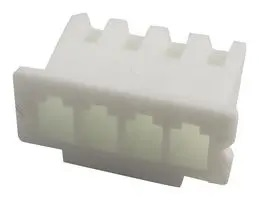
\includegraphics[scale=0.4]{pictures/connectors/XH/XHP-4.jpg}};
            \end{scope}
        }{
            \draw (0,0) rectangle (3,1.5) ;
        }{Farnell}{JST XH} {250V} {3A} 
        
        \connectorinfo{Housing}{XHP-4}{
            \tabitem \textbf{Tipo}: Plug  \\
             \tabitem \textbf{Color}: Blanco
        }

        \cline{1 - 2}
        \connectorblockinfo{Uso}{PCB - Cable - PCB}
        \connectorblockinfo{Ubicacion}{CJ}
        \pagebreak
        \hline
        \multirow{20}{*}{\makecell{Hembra \\ Header }}
        \connectordata{     
            \begin{scope}
                \clip (0,0) rectangle  +(3,1.5);
                \node[inner sep=0pt] at (1.5,0.75)
                    {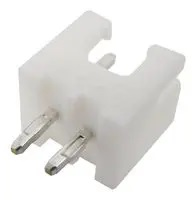
\includegraphics[scale=0.4]{pictures/connectors/XH/B2B-XH-A.jpg}};
            \end{scope}
        }{
            \draw (0,0) rectangle (3,1.5) ;
        }{Farnell}{JST XH} {250V} {3A} 
        
        \connectorinfo{Housing}{B2B-XH-A}{
            \tabitem \textbf{Tipo}: Header  \\
             \tabitem \textbf{Color}: Blanco
        }
        \connectordata{     
            \begin{scope}
                \clip (0,0) rectangle  +(3,1.5);
                \node[inner sep=0pt] at (1.5,0.75)
                    {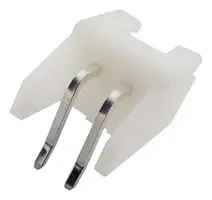
\includegraphics[scale=0.4]{pictures/connectors/XH/S2B-XH-A.jpg}};
            \end{scope}
        }{
            \draw (0,0) rectangle (3,1.5) ;
        }{Farnell}{JST XH} {250V} {3A} 
        
        \connectorinfo{Housing}{S2B-XH-A}{
            \tabitem \textbf{Tipo}: Header  \\
             \tabitem \textbf{Color}: Blanco
        }

        \connectordata{     
            \begin{scope}
                \clip (0,0) rectangle  +(3,1.5);
                \node[inner sep=0pt] at (1.5,0.75)
                    {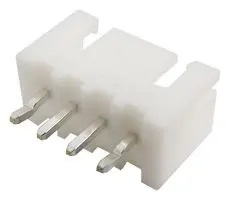
\includegraphics[scale=0.4]{pictures/connectors/XH/B4B-XH-A.jpg}};
            \end{scope}
        }{
            \draw (0,0) rectangle (3,1.5) ;
        }{Farnell}{JST XH} {250V} {3A} 
        
        \connectorinfo{Housing}{B4B-XH-A}{
            \tabitem \textbf{Tipo}: Header  \\
             \tabitem \textbf{Color}: Blanco
        }
        \connectordata{     
            \begin{scope}
                \clip (0,0) rectangle  +(3,1.5);
                \node[inner sep=0pt] at (1.5,0.75)
                    {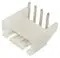
\includegraphics[scale=1]{pictures/connectors/XH/S4B-XH-A.jpg}};
            \end{scope}
        }{
            \draw (0,0) rectangle (3,1.5) ;
        }{Farnell}{JST XH} {250V} {3A} 
        
        \connectorinfo{Housing}{S4B-XH-A}{
            \tabitem \textbf{Tipo}: Header  \\
             \tabitem \textbf{Color}: Blanco
        }

        \cline{1 - 2}
        \connectorblockinfo{Uso}{PCB - Cable - PCB}
        \connectorblockinfo{Ubicacion}{CJ}

        \caption{JST XH}
        \label{tab:DcJstXH}
    \end{longtable}
}

\subsection{Conectores RJ}
% !TeX encoding = UTF-8
% !TeX spellcheck = es_ES
% !TeX root = ../ComponentCatalog.tex
%!TEX root=../ComponentCatalog.tex

%RJ45
\begin{table}[H]
    \centering
    \renewcommand\theadfont{\bfseries}
    \setlength{\tabcolsep}{10pt}
    \renewcommand{\arraystretch}{1.5}

    \begin{tabular}{|c|c|c|c|c|}
        \beginConnectorTable{RJ45}
        \multirow{3}{*}{\makecell{Macho}}
    
        \connectordata{
            \begin{scope}
                \clip (0,0) rectangle  +(3,1.5);
                \node[inner sep=0pt] at (1.5,0.75)
                    {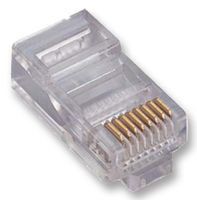
\includegraphics[scale=.1]{pictures/connectors/RJ45-nb.jpg}};
            \end{scope}
        }{
            \draw (0,0) rectangle (3,1.5) ;
        }{Amazon}{RJ45} {150V} {1.5A} 
        
        \connectorinfo{Codigo}{MTP-88-U}{
            \tabitem \textbf{Fabricante}: Multicomp
        }
        \cline{1 - 2}
        \multirow{3}{*}{\makecell{Macho}}
        \connectordata{
            \begin{scope}
                \clip (0,0) rectangle  +(3,1.5);
                \node[inner sep=0pt] at (1.5,0.75)
                    {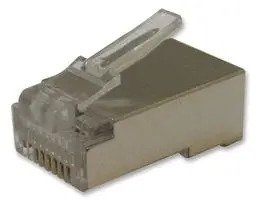
\includegraphics[scale=.1]{pictures/connectors/RJ45-b.jpg}};
            \end{scope}
        }{
            \draw (0,0) rectangle (3,1.5) ;
        }{Amazon}{RJ45} {150V} {3A}
        \connectorinfo{Codigo}{7001-8P8C-R-M}{
            \tabitem \textbf{Fabricante}: Multicomp Pro
        }
        \cline{1 - 2}
        \connectorblockinfo{Uso}{Modulos LCC OpenlCB}
        \connectorblockinfo{Ubicacion}{Terraza}
    \end{tabular}
    \caption{Conectores RJ45}
    \label{tab:RJ45}
\end{table}

%\begin{table}[H]
%    \centering
%    \renewcommand\theadfont{\bfseries}
%    \setlength{\tabcolsep}{10pt}
%    \renewcommand{\arraystretch}{1.5}


%    \begin{tabular}{c |c |c |c |c |}
%        entrada & \thead[b]{item} & \thead[b]{Recomendado} & \thead[b]{Maximo} & \thead[b]{Con Bypass} \\ 
%        \Xhline{5\arrayrulewidth}
%Entrada DCC
%        \rowcolor{Melon!15}
%        & Voltaje &14-20V & \multicolumn{2}{c|}{12-24V} \\
%        \cline{2 - 5}
%        \rowcolor{Melon!10} \cellcolor{Melon!15}
%        \multirow{-2}{*}{DCC}&Corriente & 1A & 1.5A & 2A \\ \Xhline{3\arrayrulewidth}
%Entrada Jack
%        \rowcolor{blue!15} & Voltaje & 12-20V & \multicolumn{2}{c|}{10-24V} \\
%        \cline{2 - 5}
%        \rowcolor{blue!10} \cellcolor{blue!15} \multirow{-2}{*}{ \makecell{ \cellcolor{blue!15} Jack\\ \cellcolor{blue!15} Terminal}} & Corriente & 1A & 1.5A & 3A \\
%        \Xhline{5\arrayrulewidth}
%    \end{tabular}
%    \caption{Limites de entrada}
%    \label{tab:limiteEntrada}
%\end{table}